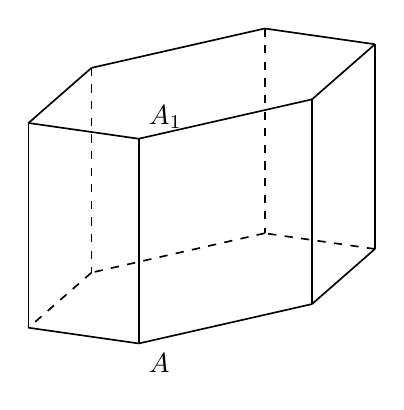
\begin{tikzpicture}[line width=.6pt, font=\normalsize]
% Top face (y around 0.6..2.0), bottom face shifted down
\coordinate (T0) at (0,0.6);
\coordinate (T1) at (2.2,1.1);
\coordinate (T2) at (3,1.8);
\coordinate (T3) at (1.6,2);
\coordinate (T4) at (-0.6,1.5);
\coordinate (T5) at (-1.4,0.8);
\coordinate (B0) at (0,-2);
\coordinate (B1) at (2.2,-1.5);
\coordinate (B2) at (3,-0.8);
\coordinate (B3) at (1.6,-0.6);
\coordinate (B4) at (-0.6,-1.1);
\coordinate (B5) at (-1.4,-1.8);
\coordinate (A1) at (0,0.6);
\coordinate (A) at (0,-2.0);
% Top face solid
\draw (T5) -- (T0);
\draw (T0) -- (T1);
\draw (T1) -- (T2);
\draw (T2) -- (T3);
\draw (T3) -- (T4);
\draw (T4) -- (T5);
% Bottom face: front solid, back dashed
\draw (B5) -- (B0);
\draw (B0) -- (B1);
\draw (B1) -- (B2);
\draw[dashed] (B2) -- (B3);
\draw[dashed] (B3) -- (B4);
\draw[dashed] (B4) -- (B5);
% Verticals: front/side solid, back dashed
\draw (T0) -- (B0);
\draw (T1) -- (B1);
\draw[dashed] (T4) -- (B4);
\draw (T5) -- (B5);
\draw (T2) -- (B2);
\draw[dashed] (T3) -- (B3);
% Labels with clearance (offset right to avoid vertical stroke)
\node[above right] at (A1) {$A_{1}$};
\node[below right] at (A) {$A$};
\end{tikzpicture}
